\section{Presentación del libro}

\begin{frame}
	\frametitle{\secname}
	\begin{minipage}{0.47\textwidth}
		\begin{figure}[ht!]
			\centering
			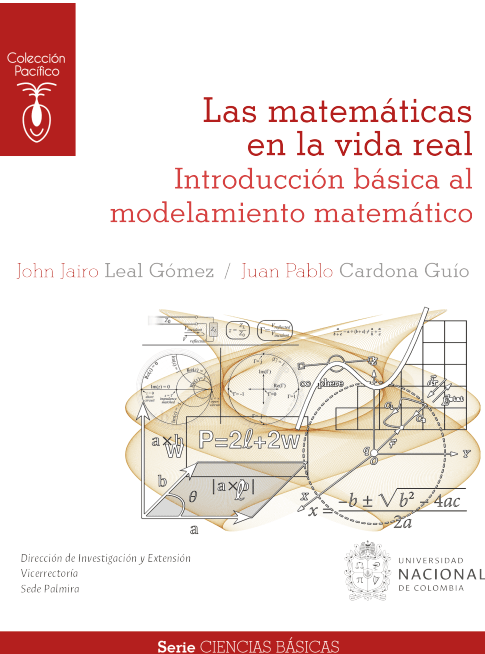
\includegraphics[height=7.7cm]{portada}
		\end{figure}
		\note{
			Los autores, John Jairo Leal y Juan Pablo Cardona les compartimos nuestro texto, y les contamos que es el producto de varios proyectos educativos de modelamiento matemático en las aulas en cursos de ingeniería.

			Una de nuestras líneas de investigación es precisamente la educación  matemática para ingeniería y lo que esperamos es que más personas y más profesionales se vinculen con aplicaciones de matemáticas y con desarrollos futuros.
		}
	\end{minipage}
	\begin{minipage}{0.5\textwidth}
		\textsc{\Large Capítulos:}

		\

		\begin{enumerate}
			\item

			      Introducción a los números reales $\mathbb{R}$.

			      \

			\item

			      Introducción a las funciones.

			      \

			\item

			      La derivada.

			      \

			\item

			      Modelamiento matemático.

			      \

			\item

			      Anexos.
		\end{enumerate}
	\end{minipage}
	\note{
		En su estructura el texto es introductorio para los primeros cursos de matemáticas, de hecho lo hemos utilizado en un curso que se llama matemáticas básicas, estudia las funciones y las derivadas y luego muestra algunos ejemplos de la vida cotidiana y cómo éstos se pueden escribir utilizando los símbolos
		matemáticos.
	}
\end{frame}

\begin{frame}
	\frametitle{\secname}
	\begin{figure}[ht!]
		\centering
		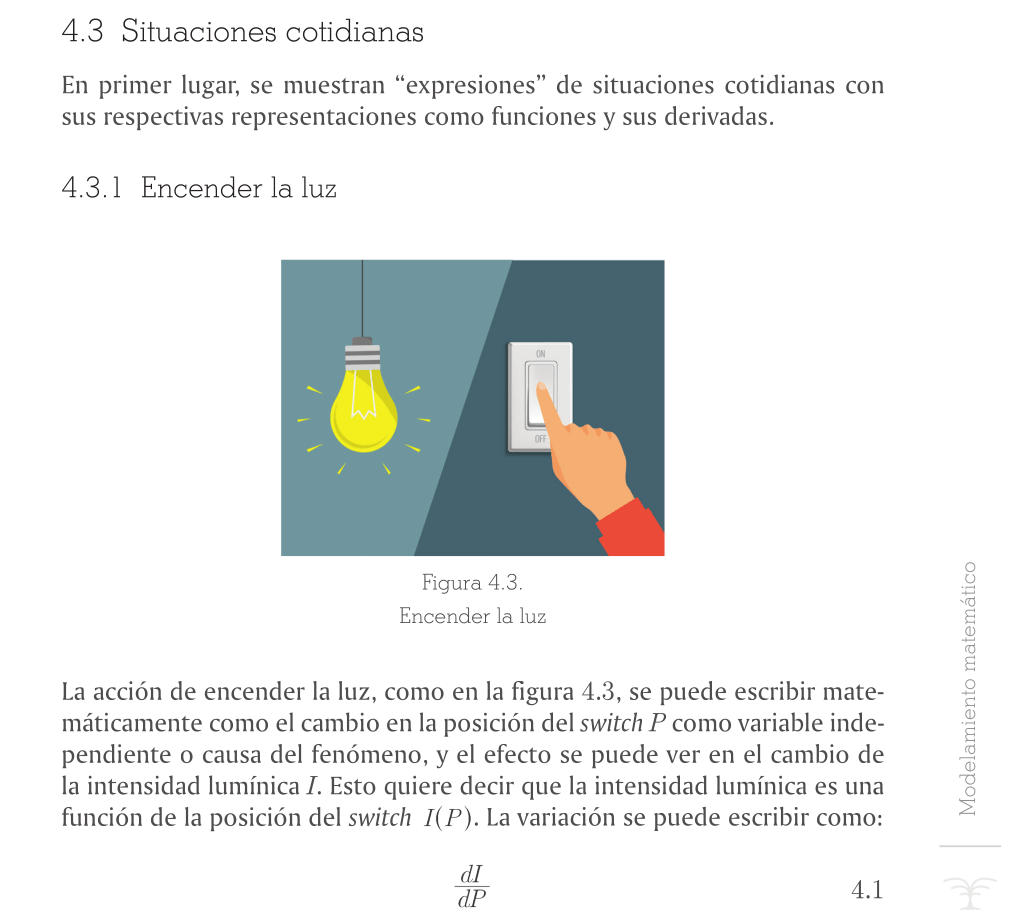
\includegraphics[height=7.8cm]{vida_cotidiana}
	\end{figure}
	\note{
		En la diapositiva se muestra una de estas situaciones diarias.
		También se tiene un anexo donde se estudia un software libre como es wxmaxima.
	}
\end{frame}